\documentclass[preview]{standalone}
\usepackage{tikz}

\begin{document}
  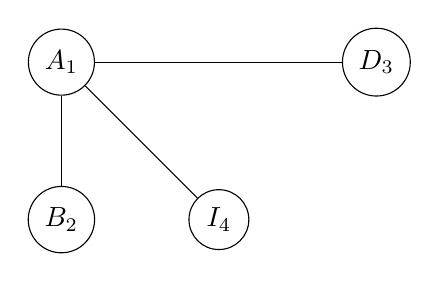
\begin{tikzpicture}
    \draw 
    (1, 3) node[circle, black, draw](B){$B_2$}
    (1, 5) node[circle, black, draw](A){$A_1$}
    (3, 3) node[circle, black, draw](I){$I_4$}
    (5, 5) node[circle, black, draw](D){$D_3$};

    \draw[-] (A) -- (B);
    \draw[-] (A) -- (I);
    \draw[-] (A) -- (D);

  \end{tikzpicture}
\end{document}
